\section{Introduction}

The Chua Circuit is an electronic circuit named after Leon Chua, who
suggested it in 1983.  It was reported by Matsumoto in 1984
\cite{Matsumoto84} that (a simplified version of) this system
exhibited chaotic behaviour in the form of a chaotic attractor,
although it is a simple autonomous circuit.

The circuit in question is shown in figure \ref{fig:circuit}.  It
contains four passive elements -- two capacitors $C_1, C_2$, one
inductor $L$ and a resistor $G$ -- and one non-linear resistor $R$.
In the original circuit the non-linearity of $R$ was given by a
three-component piecewise linear function, dependent on the voltage
over the resistor \cite{Matsumoto84,Matsumoto85,Chua86}, giving the
current through it.  We will, however, instead study a resistor with a
non-linearity that is given by the function
\begin{equation}
  \label{eq:non-linearity}
  \phi(x) = \rho x^3 - \sigma x
\end{equation}
as suggested in \cite[p. 379]{hirsch12}.  The study will also follow
the ``exploration'' given in this publication and expand on it.

\begin{figure}[h]
  \centering
  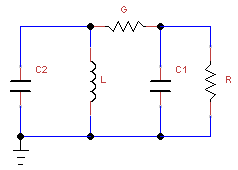
\includegraphics{chuacircuit.png}
  \caption{The Chua Circuit.  The resistor R has a non-linear dependence on the voltage.  After \cite{Matsumoto84,Matsumoto85}.}
  \label{fig:circuit}
\end{figure}

The dynamics of the original circuit can be described by the following
equations \cite[eq. (1.1)]{Matsumoto85}:
\begin{equation}
  \label{eq:dynamics}
  \left\{
    \begin{aligned}
      C_1\frac{dv_{C_1}}{dt} &= G(v_{C_2}-v_{C_1})-f(v_{C_1})\\
      C_2\frac{dv_{C_2}}{dt} &= G(v_{C_1}-v_{C_2}) + i_L\\
      L \frac{di_L}{dt} &= -v_{C_2}
    \end{aligned}
  \right.
\end{equation}
This set of equations can be rescaled to transform it into \cite[eq. (1.1)]{Chua86}:
\begin{equation}
  \label{eq:rescaling}
  \left\{
    \begin{aligned}
      \frac{dx}{d\tau} &= a(y-\phi(x))\\
      \frac{dy}{d\tau} &= x - y + z\\
      \frac{dz}{d\tau} &= -b y
    \end{aligned}
  \right.
\end{equation}
We will now, in accordance with \cite{hirsch12}, modify this circuit
by taking $\phi(x)$ as in eq. \ref{eq:non-linearity} and looking at the
following system:
\begin{equation}
  \label{eq:system}
  \left\{
    \begin{aligned}
      x' &= a(y-\phi(x))\\
      y' &= x-y+z\\
      z' &= -by
    \end{aligned}
  \right.
\end{equation}



%%% Local Variables: 
%%% mode: latex
%%% TeX-master: "chua_circuit"
%%% End: 
